\documentclass[border=6pt]{standalone}
\usepackage[T1]{fontenc}
\usepackage{lmodern}
\usepackage{amsmath,amssymb}
\usepackage{tikz}
\usetikzlibrary{arrows.meta,calc,positioning,shapes.misc,decorations.pathreplacing}
\definecolor{hyp}{RGB}{38,94,160}
\definecolor{half}{RGB}{204,110,20}
\definecolor{conj}{RGB}{176,32,40}
\definecolor{side}{RGB}{100,100,110}
\definecolor{planeA}{RGB}{232,240,250}
\definecolor{planeB}{RGB}{252,240,226}
\definecolor{planeC}{RGB}{250,232,232}

\begin{document}
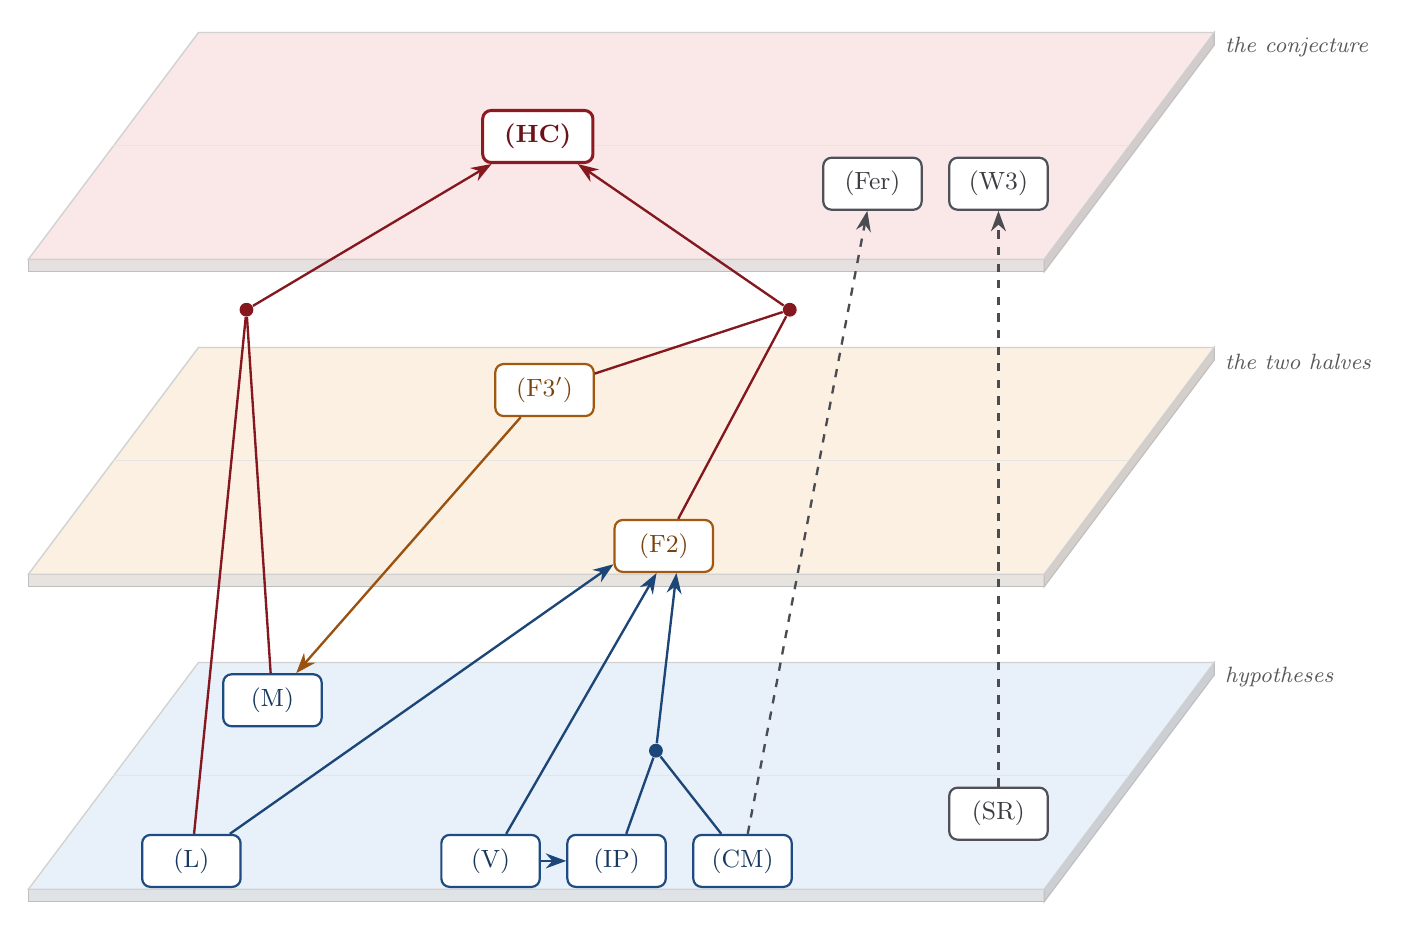
\begin{tikzpicture}[
  x={(1cm,0cm)}, y={(0.45cm,0.6cm)}, z={(0cm,1cm)},
  >={Stealth[length=2.6mm,width=1.9mm]}, font=\small,
  st/.style={rounded corners=3pt, draw=#1!80!black, fill=white,
    line width=0.8pt, minimum width=12.5mm, minimum height=6.6mm,
    inner sep=2pt, text=#1!60!black},
  imp/.style={->, line width=0.85pt, draw=#1!75!black},
  leg/.style={line width=0.85pt, draw=#1!75!black},
  dot/.style={circle, fill=#1!75!black, inner sep=0pt, minimum size=5pt},
  lab/.style={font=\footnotesize\itshape, text=black!65, anchor=west, align=left}]

% the three layers
\foreach \z/\c/\t in {0/planeA/{hypotheses},4/planeB/{the two halves},8/planeC/{the conjecture}}{
  \filldraw[fill=\c!80!black!45, draw=black!25, line width=0.4pt]
    (-1.6,-0.6,\z) -- (11.3,-0.6,\z) -- (11.3,-0.6,\z-0.16) -- (-1.6,-0.6,\z-0.16) -- cycle;
  \filldraw[fill=\c!70!black!55, draw=black!25, line width=0.4pt]
    (11.3,-0.6,\z) -- (11.3,4.2,\z) -- (11.3,4.2,\z-0.16) -- (11.3,-0.6,\z-0.16) -- cycle;
  \filldraw[fill=\c, draw=black!18, line width=0.5pt]
    (-1.6,-0.6,\z) -- (11.3,-0.6,\z) -- (11.3,4.2,\z) -- (-1.6,4.2,\z) -- cycle;
  \draw[black!10, line width=0.4pt] (-1.6,1.8,\z) -- (11.3,1.8,\z);
  \node[lab] at (11.45,3.9,\z) {\t};
}

% statements
\node[st=hyp]  (L)  at (0.2,0,0)   {(L)};
\node[st=hyp]  (M)  at (-0.3,3.4,0) {(M)};
\node[st=hyp]  (V)  at (4.0,0,0)   {(V)};
\node[st=hyp]  (IP) at (5.6,0,0)   {(IP)};
\node[st=hyp]  (CM) at (7.2,0,0)   {(CM)};
\node[st=side] (SR) at (10.0,1,0)  {(SR)};
\node[st=half] (F2) at (6.2,0,4)   {(F2)};
\node[st=half] (F3) at (3.2,3.3,4) {(F3$'$)};
\node[st=conj, line width=1.1pt, minimum width=14mm, font=\small\bfseries] (HC) at (3.7,2,8) {(HC)};
\node[st=side] (Fer) at (8.4,1,8)  {(Fer)};
\node[st=side] (W3)  at (10.0,1,8) {(W3)};

% conjunction points
\node[dot=hyp]  (C) at (5.65,1,0.8) {};
\node[dot=conj] (A) at (0.45,1,6.4) {};
\node[dot=conj] (B) at (7.35,1,6.4) {};

% implications
\draw[imp=hyp] (L) -- (F2.200);
\draw[imp=hyp] (V) -- (F2.255);
\draw[imp=hyp] (V) -- (IP);
\draw[leg=hyp] (IP) -- (C);
\draw[leg=hyp] (CM) -- (C);
\draw[imp=hyp] (C) -- (F2.295);
\draw[imp=half] (F3) -- (M);
\draw[leg=conj] (L) -- (A);
\draw[leg=conj] (M) -- (A);
\draw[imp=conj] (A) -- (HC);
\draw[leg=conj] (F2) -- (B);
\draw[leg=conj] (F3) -- (B);
\draw[imp=conj] (B) -- (HC);
\draw[imp=side, dashed] (CM) -- (Fer);
\draw[imp=side, dashed] (SR) -- (W3);

\end{tikzpicture}
\end{document}
